\documentclass[10pt,aspectratio=169,t]{beamer}

\usepackage{graphicx}
\usepackage[table]{xcolor}
\usepackage{booktabs}
\usepackage{array}
\usepackage{url}
\usepackage{hyperref}

\usetheme{Berlin}
\usecolortheme{default}
\useinnertheme{rectangles}
\useoutertheme{infolines}

\definecolor{HackBlue}{HTML}{3b82f6}
\definecolor{HackPurple}{HTML}{8b5cf6}
\definecolor{HackGreen}{HTML}{10b981}
\definecolor{HackOrange}{HTML}{f97316}
\definecolor{HackDark}{HTML}{0f172a}
\definecolor{SupabaseGreen}{HTML}{3ecf8e}
\definecolor{GCPBlue}{HTML}{4285f4}

\setbeamertemplate{footline}[frame number]
\setbeamertemplate{navigation symbols}{}

\usepackage{tikz}
\usetikzlibrary{arrows,shapes.geometric,positioning,calc,shadows}
\tikzset{
  >=stealth,
  node distance=1.5cm,
  service/.style={
    draw,
    rounded corners=8pt,
    minimum width=2.8cm,
    minimum height=1cm,
    align=center,
    font=\sffamily\small\bfseries,
    drop shadow={shadow xshift=2pt, shadow yshift=-2pt, opacity=0.1}
  },
  github/.style={service, fill=HackDark, text=white},
  vercel/.style={service, fill=black, text=white},
  supabase/.style={service, fill=SupabaseGreen, text=white},
  gcp/.style={service, fill=GCPBlue, text=white},
  verda/.style={service, fill=HackPurple, text=white},
  user/.style={service, fill=HackOrange, text=white},
  arrow/.style={->, thick, draw=gray!60},
  dashed-arrow/.style={->, thick, draw=gray!60, dash pattern=on 4pt off 2pt}
}

\title[]{Hackathon Monorepo Template}
\subtitle[]{Vercel + Supabase + Google Cloud + Verda}
\author[]{PlayerPlanet Team}
\institute[]{\textbf{HackMIT 2026}}

\begin{document}

% SLIDE 1: Title
{
  \setbeamertemplate{background}{
    \begin{tikzpicture}[overlay,remember picture]
      \fill[HackDark] (current page.south west) rectangle (current page.north east);
    \end{tikzpicture}
  }
  \begin{frame}[plain,noframenumbering]
    \vspace{1.5cm}
    \titlepage
    \vfill
    \begin{columns}
      \begin{column}{0.25\paperwidth}\centering\textbf{Vercel}\\\footnotesize Frontend + API\end{column}
      \begin{column}{0.25\paperwidth}\centering\textbf{Supabase}\\\footnotesize Postgres + Auth\end{column}
      \begin{column}{0.25\paperwidth}\centering\textbf{Cloud Run}\\\footnotesize Inference Service\end{column}
      \begin{column}{0.25\paperwidth}\centering\textbf{Verda}\\\footnotesize Inference API\end{column}
    \end{columns}
  \end{frame}
}

% SLIDE 2: What Is This?
\begin{frame}{What Is This Template?}

  \begin{block}{Problem}
    \begin{itemize}
      \item Hackathons need \textbf{fast iteration}: idea to deployed in minutes
      \item But teams waste the first 2--4 hours on infrastructure setup
      \item Cookiecutter templates risk disqualification if code exists before the event
    \end{itemize}
  \end{block}

  \vfill

  \begin{block}{Solution}
    \begin{itemize}
      \item This is a \textbf{cookiecutter template} --- generates a fresh project at hackathon start
      \item Every generated file is \alert{infrastructure only}, annotated with \texttt{TODO} for your code
      \item One timestamped commit proves all code was written during the event
      \item Pre-configured CI/CD deploys automatically on every push
    \end{itemize}
  \end{block}

  \vfill

  \begin{alertblock}{Key Guarantee}
    The generated repository has exactly \textbf{one commit} (the generation itself).
    No ancestral history. No pre-written feature code.
  \end{alertblock}

\end{frame}

% SLIDE 3: The Stack
\begin{frame}{The Stack}

  \begin{center}
    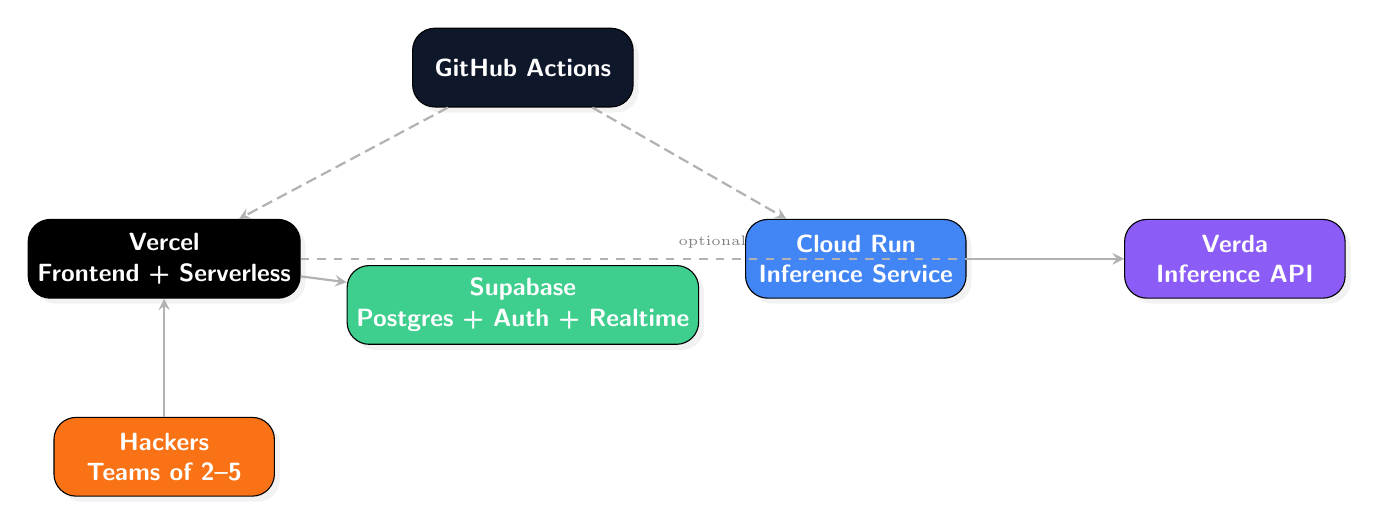
\begin{tikzpicture}[node distance=2cm]
      \node[github] (github) {GitHub Actions};
      \node[vercel, below left=of github] (vercel) {Vercel\\\small Frontend + Serverless};
      \node[supabase, below=of github] (supabase) {Supabase\\\small Postgres + Auth + Realtime};
      \node[gcp, below right=of github] (gcp) {Cloud Run\\\small Inference Service};
      \node[verda, right=of gcp] (verda) {Verda\\\small Inference API};
      \node[user, below=of vercel, yshift=0.5cm] (user) {Hackers\\\small Teams of 2--5};

      \draw[dashed-arrow] (github) -- (vercel);
      \draw[dashed-arrow] (github) -- (gcp);
      \draw[arrow] (vercel) -- (supabase);
      \draw[arrow] (gcp) -- (verda);
      \draw[arrow, dashed] (vercel) -- (verda) node[midway, above, font=\tiny, gray] {optional};
      \draw[arrow] (user) -- (vercel);
    \end{tikzpicture}
  \end{center}

  \begin{table}
    \centering
    \small
    \begin{tabular}{lll}
      \toprule
      \textbf{Layer} & \textbf{Technology} & \textbf{Deploys via} \\
      \midrule
      Frontend + API routes & Next.js 14 on Vercel & GitHub Actions (Vercel CLI) \\
      Database + Auth + Realtime & Supabase (managed Postgres) & Manual or CLI \\
      Inference Service & Node.js + Express on Cloud Run & Cloud Build + Cloud Run \\
      AI/ML Inference & Verda API (external) & Called by Cloud Run \\
      CI/CD Orchestration & GitHub Actions & Push to branch \\
      \bottomrule
    \end{tabular}
  \end{table}

\end{frame}

% SLIDE 4: Service Boundaries
\begin{frame}{Service Boundaries --- What Goes Where?}

  \begin{table}
    \centering
    \small
    \begin{tabular}{p{3.5cm}p{4cm}p{2.5cm}}
      \toprule
      \textbf{What} & \textbf{Where} & \textbf{Why} \\
      \midrule
      Next.js frontend (SSR, ISR) & \cellcolor{HackBlue} Vercel & Zero-config edge CDN, preview deploys per PR \\
      Vercel serverless functions & \cellcolor{HackBlue} Vercel & Tight frontend integration, fast iteration \\
      User-facing API routes & \cellcolor{HackBlue} Vercel & Same Vercel project, shared domain \\
      Heavy backend / async tasks & \cellcolor{GCPBlue} Cloud Run & GPU workloads, Verda proxy, long-running jobs \\
      Database + Auth + Realtime & \cellcolor{SupabaseGreen} Supabase & Managed Postgres, no ops overhead \\
      Inference / LLM calls & \cellcolor{HackPurple} Verda & Keep API key secret, centralized access \\
      CI/CD orchestration & \cellcolor{HackDark} GitHub Actions & Branch-based promotion, secret injection \\
      \bottomrule
    \end{tabular}
  \end{table}

  \vfill

  \begin{block}{Why Not Supabase Edge Functions for Inference?}
    \begin{itemize}
      \item Supabase Edge Functions are stateless and time-limited (max 60s)
      \item Verda inference calls can take minutes for large prompts
      \item Cloud Run supports min-instances = 1 (no cold starts) + 60s timeout
      \item Cloud Run container is portable (Dockerfile works locally and on GCP)
    \end{itemize}
  \end{block}

\end{frame}

% SLIDE 5: CI/CD Pipeline
\begin{frame}{CI/CD Pipeline (GitHub Actions)}

  \begin{columns}

    \begin{column}{0.5\paperwidth}

      \textbf{Workflows:}

      \begin{enumerate}
        \item \texttt{ci.yml} --- every push/PR

          \quad Lint + TypeScript check + test

          \quad 5 min timeout, cancels in-progress

        \item \texttt{deploy-vercel.yml} --- every push to \texttt{dev/staging/main}

          \quad vercel pull -> vercel build -> vercel deploy

          \quad Branch-based env (preview on PR)

        \item \texttt{deploy-cloudrun.yml} --- push to \texttt{staging/main}

          \quad Cloud Build -> Artifact Registry -> Cloud Run

          \quad Secrets injected at deploy time

        \item \texttt{deploy-all.yml} --- orchestrated

          \quad Vercel -> Cloud Run (sequential)
      \end{enumerate}

    \end{column}

    \begin{column}{0.45\paperwidth}

      \begin{block}{Secrets (GitHub Secrets)}
        \ttfamily\scriptsize
        \begin{tabular}{l}
          VERCEL\_TOKEN\\
          VERCEL\_ORG\_ID\\
          VERCEL\_PROJECT\_ID\\
          NEXT\_PUBLIC\_SUPABASE\_URL\\
          NEXT\_PUBLIC\_SUPABASE\_ANON\_KEY\\
          SUPABASE\_SERVICE\_ROLE\_KEY\\
          GCP\_SA\_KEY (base64-encoded)\\
          VERDA\_API\_KEY\\
          VERDA\_API\_URL\\
          GCP\_PROJECT\_ID (GitHub Variable)
        \end{tabular}
      \end{block}

      \begin{block}{Deploy Triggers}
        \begin{tabular}{ll}
          \toprule
          Branch & Deploys \\
          \midrule
          feature/* & Vercel preview (PR) \\
          dev & Vercel dev \\
          staging & Vercel staging + Cloud Run \\
          main & Vercel prod + Cloud Run prod \\
          \bottomrule
        \end{tabular}
      \end{block}

    \end{column}

  \end{columns}

\end{frame}

% SLIDE 6: Monorepo Structure
\begin{frame}{Monorepo Structure}

  \begin{columns}

    \begin{column}{0.55\paperwidth}

      \begin{block}{Monorepo Layout}
        \ttfamily\scriptsize
        cookiecutter-hackathon-template/\\
        \hspace{1em}.github/workflows/\\
        \hspace{2em}ci.yml, deploy-vercel.yml,\\
        \hspace{2em}deploy-cloudrun.yml, deploy-all.yml\\
        \hspace{1em}apps/\\
        \hspace{2em}web/ (Next.js), api/ (Vercel fn)\\
        \hspace{1em}services/\\
        \hspace{2em}inference/ (Cloud Run)\\
        \hspace{1em}packages/\\
        \hspace{2em}shared/, db/\\
        \hspace{1em}supabase/migrations/\\
        \hspace{1em}turbo.json, package.json
      \end{block}

    \end{column}

    \begin{column}{0.4\paperwidth}

      \begin{block}{npm workspaces}
        \ttfamily\scriptsize
        \{ "workspaces": ["apps/*", "services/*", "packages/*"] \}
      \end{block}

      \begin{block}{Turbo pipeline}
        Build runs topologically (dependsOn \texttt{\string^build}). Dev is persistent with cache disabled.
      \end{block}

      \begin{block}{Tools}
        \begin{itemize}
          \item Turborepo for build orchestration
          \item npm workspaces for package management
          \item GitHub Actions for CI/CD
        \end{itemize}
      \end{block}

    \end{column}

  \end{columns}

\end{frame}

% SLIDE 7: Inference Service
\begin{frame}{Inference Service --- Cloud Run + Verda}

  \begin{columns}

    \begin{column}{0.45\paperwidth}

      \begin{block}{Dockerfile (Multi-stage)}
        \ttfamily\scriptsize
        \begin{verbatim}
FROM node:20-alpine AS base
WORKDIR /app
FROM base AS deps
COPY package*.json ./
RUN npm ci --omit=dev
FROM base AS builder
COPY --from=deps /app/node_modules ./
COPY . . && npm run build
FROM base AS runner
ENV NODE_ENV=production
COPY --from=builder /app/dist ./dist
COPY --from=builder /app/package*.json ./
EXPOSE 3000
CMD ["node", "dist/index.js"]
        \end{verbatim}
      \end{block}

    \end{column}

    \begin{column}{0.5\paperwidth}

      \begin{block}{Inference Skeleton (Node.js + Express)}
        \ttfamily\scriptsize
        \begin{verbatim}
// GENERATED by cookiecutter
import express, { Request, Response } from 'express';
const app = express();
app.use(express.json());
app.get('/health', (_req, res) => {
  res.json({ status: 'ok' });
});
app.post('/api/inference', async (req, res) => {
  // TODO (hackathon): implement logic here
  res.status(501).json({ error: 'Not implemented' });
});
app.listen(3000, '0.0.0.0', () => { });
        \end{verbatim}
      \end{block}

      \begin{alertblock}{Secrets Injection}
        At deploy time, secrets are injected via \texttt{--set-env-vars} (not baked into image):
        \ttfamily\scriptsize
        gcloud run deploy inference-service --set-env-vars VERDA\_API\_KEY=\$Secrets.VERDA\_API\_KEY
      \end{alertblock}

    \end{column}

  \end{columns}

\end{frame}

% SLIDE 8: Supabase Schema
\begin{frame}{Supabase --- Database Schema}

  \begin{columns}

    \begin{column}{0.55\paperwidth}

      \begin{block}{Migration File (at hackathon start)}
        \ttfamily\scriptsize
        \begin{verbatim}
-- GENERATED by cookiecutter
CREATE EXTENSION IF NOT EXISTS "uuid-ossp";
-- TODO (hackathon): add your tables here
-- CREATE TABLE public.my_table (
--   id UUID PRIMARY KEY DEFAULT uuid_generate_v4(),
--   name TEXT NOT NULL
-- );
-- TODO (hackathon): add RLS policies
-- ALTER TABLE public.my_table ENABLE ROW LEVEL SECURITY;
        \end{verbatim}
      \end{block}

    \end{column}

    \begin{column}{0.4\paperwidth}

      \begin{block}{Supabase Client}
        \ttfamily\scriptsize
        \begin{verbatim}
// GENERATED by cookiecutter
import { createClient } from '@supabase/supabase-js';
const supabaseUrl = process.env.NEXT_PUBLIC_SUPABASE_URL ?? '';
const supabaseAnonKey = process.env.NEXT_PUBLIC_SUPABASE_ANON_KEY ?? '';
export const supabase = createClient(supabaseUrl, supabaseAnonKey);
// TODO (hackathon): add your DB ops
        \end{verbatim}
      \end{block}

      \begin{block}{Why Not Prisma?}
        \begin{itemize}
          \item Supabase's JS client is auto-generated from Postgres schema
          \item No schema drift between prisma schema and actual DB
          \item Simpler hackathon workflow: just write SQL
        \end{itemize}
      \end{block}

    \end{column}

  \end{columns}

\end{frame}

% SLIDE 9: What to Implement
\begin{frame}{What to Implement During the Hackathon}

  \begin{columns}

    \begin{column}{0.5\paperwidth}

      \begin{block}{Frontend (Next.js)}
        \ttfamily\scriptsize
        \begin{verbatim}
export default function Home() {
  return (
    <main>
      <h1>project_name</h1>
      <p>Start coding here!</p>
      {/* TODO: build your UI */}
    </main>
  );
}
        \end{verbatim}
      \end{block}

      \begin{block}{API Routes (Vercel Functions)}
        \ttfamily\scriptsize
        \begin{verbatim}
export default async function handler(
  req, res
) {
  // TODO (hackathon): implement
  res.status(501).json({ error: 'Not implemented' });
}
        \end{verbatim}
      \end{block}

    \end{column}

    \begin{column}{0.45\paperwidth}

      \begin{block}{Shared Types}
        \ttfamily\scriptsize
        \begin{verbatim}
// GENERATED by cookiecutter
export type HackathonType = never;
// TODO (hackathon): add your Zod schemas
// export const MySchema = z.object({ ... });
        \end{verbatim}
      \end{block}

      \begin{block}{Database Operations}
        \ttfamily\scriptsize
        \begin{verbatim}
// TODO (hackathon): add DB operations
// export async function getProjects() {
//   return supabase.from('projects').select('*');
// }
        \end{verbatim}
      \end{block}

      \begin{alertblock}{The Rule}
        Every file is annotated with \texttt{TODO (hackathon)}. All code with dates before the event = disqualification risk.
      \end{alertblock}

    \end{column}

  \end{columns}

\end{frame}

% SLIDE 10: Quick Start
\begin{frame}{Quick Start (Do at Hackathon Event)}

  \begin{block}{Step 1: Generate the project}
    \ttfamily\scriptsize
    cookiecutter gh:PlayerPlanet/cookiecutter-hackathon-template --no-input
  \end{block}

  \begin{block}{Step 2: Initialize git}
    \ttfamily\scriptsize
    cd my-project \&\& git init \&\& git add . \&\& git commit -m "Scaffold from template"
  \end{block}

  \begin{block}{Step 3: Configure secrets}
    \ttfamily\scriptsize
    cp .env.example .env.local  \&\&  add keys to GitHub Secrets
  \end{block}

  \begin{block}{Step 4: Test the pipeline}
    \ttfamily\scriptsize
    git checkout -b dev \&\& git push origin dev
  \end{block}

  \begin{block}{Step 5: Start building}
    See Slide 9 for where to write code. Target: less than 60 minutes from generation to first deployed preview.
  \end{block}

\end{frame}

% SLIDE 11: Troubleshooting
\begin{frame}{Troubleshooting}

  \begin{columns}

    \begin{column}{0.5\paperwidth}

      \begin{block}{Cloud Run deployment fails}
        \begin{itemize}
          \item GCP SA needs Cloud Run Admin + Artifact Registry Writer roles
          \item Verify GCP\_PROJECT\_ID GitHub Variable matches your GCP project exactly
          \item Encode SA JSON: base64 -i key.json | tr -d '$\backslash$n'
        \end{itemize}
      \end{block}

      \begin{block}{Vercel build fails}
        \begin{itemize}
          \item NEXT\_PUBLIC\_* vars must be in Vercel dashboard, not only .env.local
          \item Run vercel pull to fetch env vars from Vercel
        \end{itemize}
      \end{block}

    \end{column}

    \begin{column}{0.45\paperwidth}

      \begin{block}{Supabase connection issues}
        \begin{itemize}
          \item URL must be full: https://abc123.supabase.co, not just abc123
          \item RLS policies may be blocking queries --- check in Supabase dashboard
        \end{itemize}
      \end{block}

      \begin{block}{GitHub Actions secrets not found}
        \begin{itemize}
          \item Secrets go in Settings -> Secrets -> Actions
          \item GCP\_PROJECT\_ID goes in Variables (not Secrets)
        \end{itemize}
      \end{block}

    \end{column}

  \end{columns}

\end{frame}

% SLIDE 12: End
{
  \setbeamertemplate{background}{
    \fill[HackDark] (current page.south west) rectangle (current page.north east);
  }
  \begin{frame}[plain,noframenumbering]

    \centering
    \vspace{2cm}

    {\LARGE Go build something.}

    \vspace{2cm}

    \begin{columns}
      \begin{column}{0.33\paperwidth}\centering
        {\large GitHub}\\
        \vspace{0.3em}github.com/PlayerPlanet/\\
        cookiecutter-hackathon-template
      \end{column}
      \begin{column}{0.33\paperwidth}\centering
        {\large Vercel}\\
        \vspace{0.3em}Frontend + API
      \end{column}
      \begin{column}{0.33\paperwidth}\centering
        {\large Supabase}\\
        \vspace{0.3em}Database + Auth
      \end{column}
    \end{columns}

    \vspace{2cm}

    \begin{beamercolorbox}[wd=\paperwidth,center,ht=1cm,dp=0.5cm]{palette primary}
      \textbf{Good luck, have fun, ship fast.}
    \end{beamercolorbox}

  \end{frame}
}

\end{document}